\section{Spark::Sp\-Copy\-To\-Texture3d\-Fb Class Reference}
\label{classSpark_1_1SpCopyToTexture3dFb}\index{Spark::SpCopyToTexture3dFb@{Spark::SpCopyToTexture3dFb}}
{\tt \#include $<$Sp\-Copy\-To\-Texture3d\-Fb.h$>$}

Inheritance diagram for Spark::Sp\-Copy\-To\-Texture3d\-Fb:\begin{figure}[H]
\begin{center}
\leavevmode
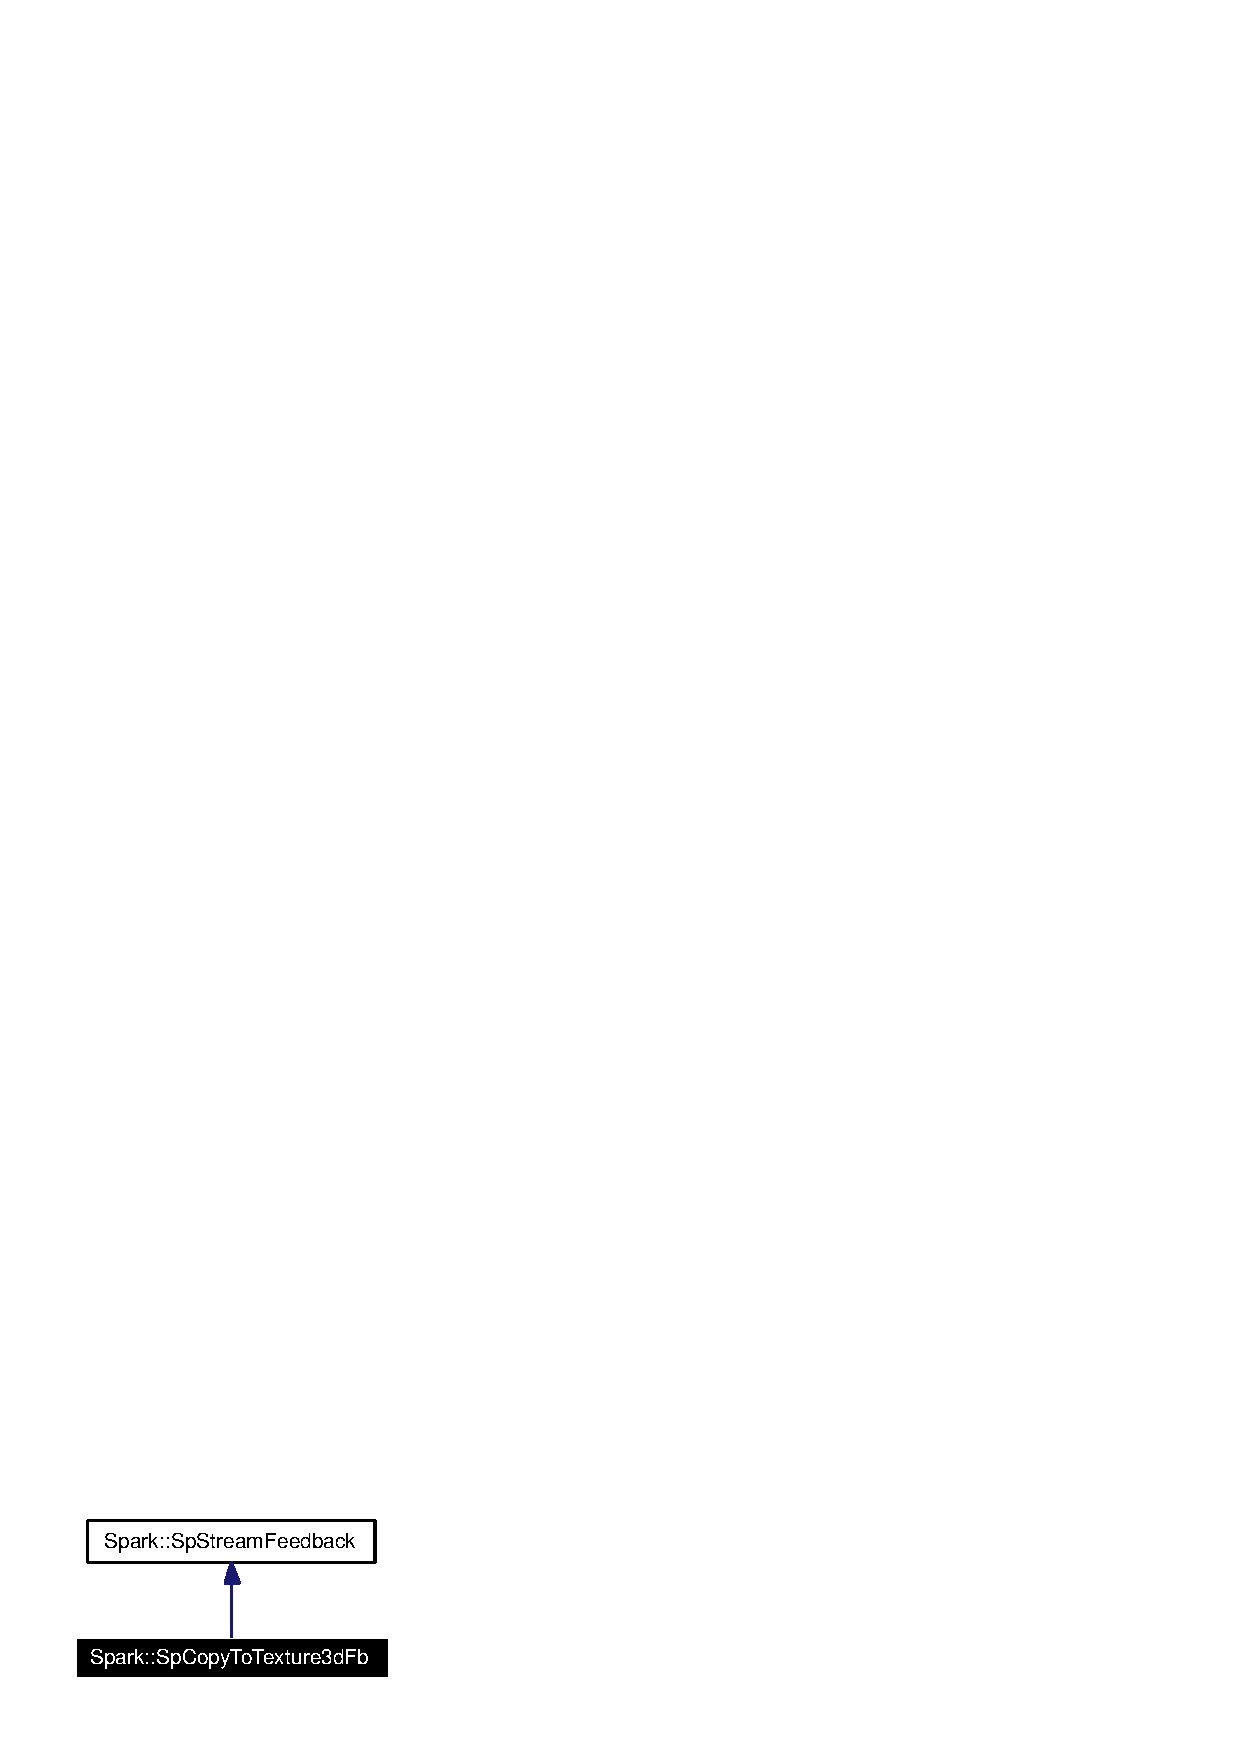
\includegraphics[width=93pt]{classSpark_1_1SpCopyToTexture3dFb__inherit__graph}
\end{center}
\end{figure}
Collaboration diagram for Spark::Sp\-Copy\-To\-Texture3d\-Fb:\begin{figure}[H]
\begin{center}
\leavevmode
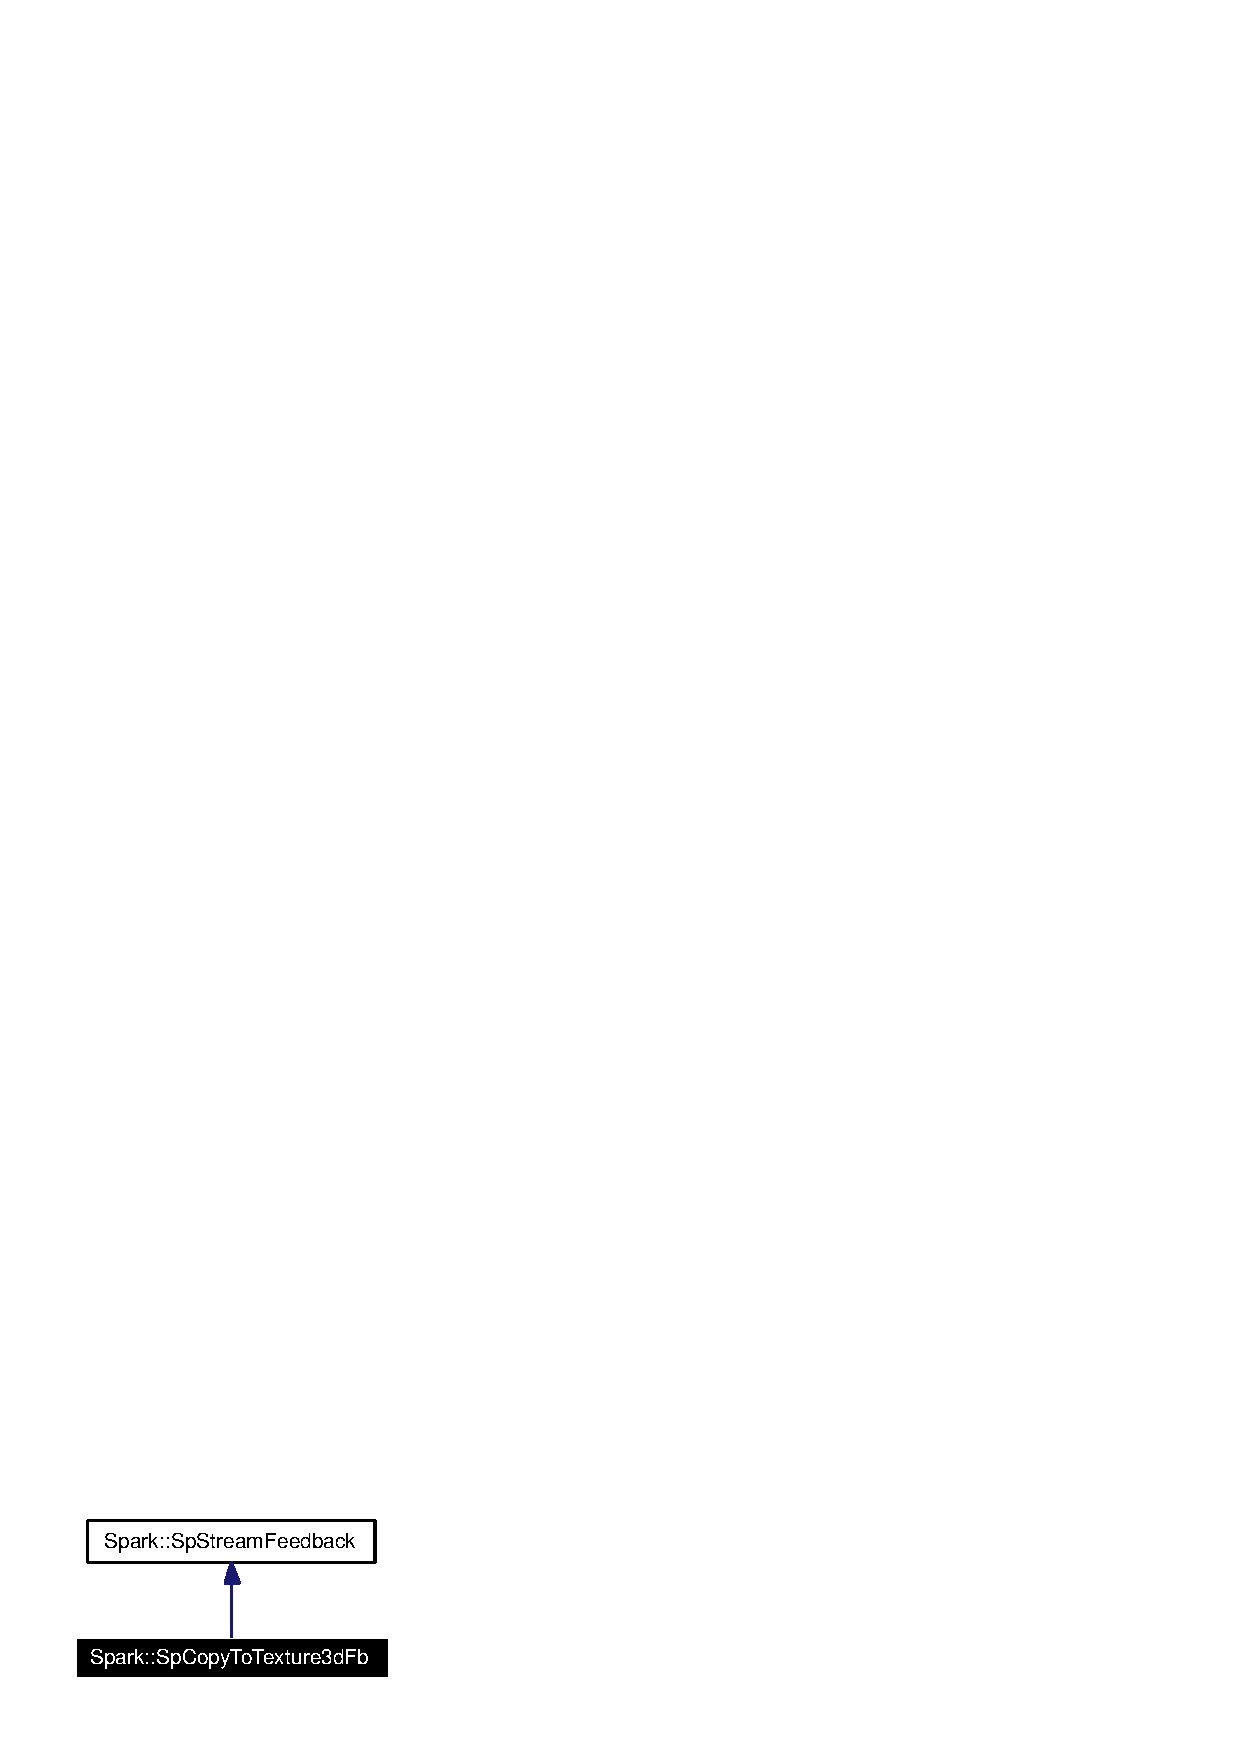
\includegraphics[width=93pt]{classSpark_1_1SpCopyToTexture3dFb__coll__graph}
\end{center}
\end{figure}


\subsection{Detailed Description}
Sliced 3D Copy To Texture (CTT) feedback mechanism via Open\-GL. 

Definition at line 33 of file Sp\-Copy\-To\-Texture3d\-Fb.h.\subsection*{Public Member Functions}
\begin{CompactItemize}
\item 
{\bf Sp\-Copy\-To\-Texture3d\-Fb} (GLuint ui\-Texture\-Id=0, int i\-X=0, int i\-Y=0, int i\-Width=0, int i\-Height=0, int i\-Depth=0, int i\-Offset\-X=0, int i\-Offset\-Y=0, int i\-Offset\-Z=0, bool b\-Enable\-Copy=true)
\begin{CompactList}\small\item\em Construction:. \item\end{CompactList}\item 
{\bf $\sim$Sp\-Copy\-To\-Texture3d\-Fb} ()
\item 
virtual void {\bf set\-Output\-Texture} (unsigned int ui\-Texture\-Id, int i\-Width, int i\-Height, int i\-Depth)
\begin{CompactList}\small\item\em Inherited Methods:. \item\end{CompactList}\item 
virtual void {\bf update\-Output} ()
\item 
void {\bf set\-Output\-Rectangle} (int i\-X, int i\-Y, int i\-Width, int i\-Height, int i\-Offset\-X, int i\-Offset\-Y, int i\-Offset\-Z)
\begin{CompactList}\small\item\em Operations:. \item\end{CompactList}\item 
void {\bf set\-Output\-Slice} (int i\-Offset\-Z)
\item 
void {\bf set\-Viewport} ()
\item 
void {\bf bind\-Output\-Texture} () const
\item 
void {\bf set\-Enable\-Copy} (bool b\-Enable)
\begin{CompactList}\small\item\em Access Methods:. \item\end{CompactList}\item 
bool {\bf get\-Enable\-Copy} () const
\end{CompactItemize}
\subsection*{Protected Attributes}
\begin{CompactItemize}
\item 
GLuint {\bf m\_\-ui\-Output\-Texture\-Id}
\begin{CompactList}\small\item\em Internal Data:. \item\end{CompactList}\item 
int {\bf m\_\-i\-Offset\-X}
\item 
int {\bf m\_\-i\-Offset\-Y}
\item 
int {\bf m\_\-i\-Offset\-Z}
\item 
int {\bf m\_\-i\-X}
\item 
int {\bf m\_\-i\-Y}
\item 
int {\bf m\_\-i\-Width}
\item 
int {\bf m\_\-i\-Height}
\item 
int {\bf m\_\-i\-Depth}
\item 
int {\bf m\_\-i\-Old\-Viewport} [4]
\item 
bool {\bf m\_\-b\-Enable\-Copy}
\end{CompactItemize}


\subsection{Constructor \& Destructor Documentation}
\index{Spark::SpCopyToTexture3dFb@{Spark::Sp\-Copy\-To\-Texture3d\-Fb}!SpCopyToTexture3dFb@{SpCopyToTexture3dFb}}
\index{SpCopyToTexture3dFb@{SpCopyToTexture3dFb}!Spark::SpCopyToTexture3dFb@{Spark::Sp\-Copy\-To\-Texture3d\-Fb}}
\subsubsection{\setlength{\rightskip}{0pt plus 5cm}Spark::Sp\-Copy\-To\-Texture3d\-Fb::Sp\-Copy\-To\-Texture3d\-Fb (GLuint {\em ui\-Texture\-Id} = {\tt 0}, int {\em i\-X} = {\tt 0}, int {\em i\-Y} = {\tt 0}, int {\em i\-Width} = {\tt 0}, int {\em i\-Height} = {\tt 0}, int {\em i\-Depth} = {\tt 0}, int {\em i\-Offset\-X} = {\tt 0}, int {\em i\-Offset\-Y} = {\tt 0}, int {\em i\-Offset\-Z} = {\tt 0}, bool {\em b\-Enable\-Copy} = {\tt true})\hspace{0.3cm}{\tt  [inline]}}\label{classSpark_1_1SpCopyToTexture3dFb_a0}


Construction:. 

Definition at line 39 of file Sp\-Copy\-To\-Texture3d\-Fb.h.

References m\_\-b\-Enable\-Copy, m\_\-i\-Depth, m\_\-i\-Height, m\_\-i\-Offset\-X, m\_\-i\-Offset\-Y, m\_\-i\-Offset\-Z, m\_\-i\-Width, m\_\-i\-X, m\_\-i\-Y, and m\_\-ui\-Output\-Texture\-Id.\index{Spark::SpCopyToTexture3dFb@{Spark::Sp\-Copy\-To\-Texture3d\-Fb}!~SpCopyToTexture3dFb@{$\sim$SpCopyToTexture3dFb}}
\index{~SpCopyToTexture3dFb@{$\sim$SpCopyToTexture3dFb}!Spark::SpCopyToTexture3dFb@{Spark::Sp\-Copy\-To\-Texture3d\-Fb}}
\subsubsection{\setlength{\rightskip}{0pt plus 5cm}Spark::Sp\-Copy\-To\-Texture3d\-Fb::$\sim${\bf Sp\-Copy\-To\-Texture3d\-Fb} ()\hspace{0.3cm}{\tt  [inline]}}\label{classSpark_1_1SpCopyToTexture3dFb_a1}


Definition at line 59 of file Sp\-Copy\-To\-Texture3d\-Fb.h.

\subsection{Member Function Documentation}
\index{Spark::SpCopyToTexture3dFb@{Spark::Sp\-Copy\-To\-Texture3d\-Fb}!bindOutputTexture@{bindOutputTexture}}
\index{bindOutputTexture@{bindOutputTexture}!Spark::SpCopyToTexture3dFb@{Spark::Sp\-Copy\-To\-Texture3d\-Fb}}
\subsubsection{\setlength{\rightskip}{0pt plus 5cm}void Spark::Sp\-Copy\-To\-Texture3d\-Fb::bind\-Output\-Texture () const\hspace{0.3cm}{\tt  [inline]}}\label{classSpark_1_1SpCopyToTexture3dFb_a7}


Definition at line 124 of file Sp\-Copy\-To\-Texture3d\-Fb.h.

References m\_\-ui\-Output\-Texture\-Id.\index{Spark::SpCopyToTexture3dFb@{Spark::Sp\-Copy\-To\-Texture3d\-Fb}!getEnableCopy@{getEnableCopy}}
\index{getEnableCopy@{getEnableCopy}!Spark::SpCopyToTexture3dFb@{Spark::Sp\-Copy\-To\-Texture3d\-Fb}}
\subsubsection{\setlength{\rightskip}{0pt plus 5cm}bool Spark::Sp\-Copy\-To\-Texture3d\-Fb::get\-Enable\-Copy () const\hspace{0.3cm}{\tt  [inline]}}\label{classSpark_1_1SpCopyToTexture3dFb_a9}


Definition at line 136 of file Sp\-Copy\-To\-Texture3d\-Fb.h.

References m\_\-b\-Enable\-Copy.\index{Spark::SpCopyToTexture3dFb@{Spark::Sp\-Copy\-To\-Texture3d\-Fb}!setEnableCopy@{setEnableCopy}}
\index{setEnableCopy@{setEnableCopy}!Spark::SpCopyToTexture3dFb@{Spark::Sp\-Copy\-To\-Texture3d\-Fb}}
\subsubsection{\setlength{\rightskip}{0pt plus 5cm}void Spark::Sp\-Copy\-To\-Texture3d\-Fb::set\-Enable\-Copy (bool {\em b\-Enable})\hspace{0.3cm}{\tt  [inline]}}\label{classSpark_1_1SpCopyToTexture3dFb_a8}


Access Methods:. 

Definition at line 133 of file Sp\-Copy\-To\-Texture3d\-Fb.h.

References m\_\-b\-Enable\-Copy.\index{Spark::SpCopyToTexture3dFb@{Spark::Sp\-Copy\-To\-Texture3d\-Fb}!setOutputRectangle@{setOutputRectangle}}
\index{setOutputRectangle@{setOutputRectangle}!Spark::SpCopyToTexture3dFb@{Spark::Sp\-Copy\-To\-Texture3d\-Fb}}
\subsubsection{\setlength{\rightskip}{0pt plus 5cm}void Spark::Sp\-Copy\-To\-Texture3d\-Fb::set\-Output\-Rectangle (int {\em i\-X}, int {\em i\-Y}, int {\em i\-Width}, int {\em i\-Height}, int {\em i\-Offset\-X}, int {\em i\-Offset\-Y}, int {\em i\-Offset\-Z})\hspace{0.3cm}{\tt  [inline]}}\label{classSpark_1_1SpCopyToTexture3dFb_a4}


Operations:. 

Definition at line 100 of file Sp\-Copy\-To\-Texture3d\-Fb.h.

References m\_\-i\-Height, m\_\-i\-Offset\-X, m\_\-i\-Offset\-Y, m\_\-i\-Offset\-Z, m\_\-i\-Width, m\_\-i\-X, and m\_\-i\-Y.\index{Spark::SpCopyToTexture3dFb@{Spark::Sp\-Copy\-To\-Texture3d\-Fb}!setOutputSlice@{setOutputSlice}}
\index{setOutputSlice@{setOutputSlice}!Spark::SpCopyToTexture3dFb@{Spark::Sp\-Copy\-To\-Texture3d\-Fb}}
\subsubsection{\setlength{\rightskip}{0pt plus 5cm}void Spark::Sp\-Copy\-To\-Texture3d\-Fb::set\-Output\-Slice (int {\em i\-Offset\-Z})\hspace{0.3cm}{\tt  [inline]}}\label{classSpark_1_1SpCopyToTexture3dFb_a5}


Definition at line 113 of file Sp\-Copy\-To\-Texture3d\-Fb.h.

References m\_\-i\-Offset\-X.\index{Spark::SpCopyToTexture3dFb@{Spark::Sp\-Copy\-To\-Texture3d\-Fb}!setOutputTexture@{setOutputTexture}}
\index{setOutputTexture@{setOutputTexture}!Spark::SpCopyToTexture3dFb@{Spark::Sp\-Copy\-To\-Texture3d\-Fb}}
\subsubsection{\setlength{\rightskip}{0pt plus 5cm}virtual void Spark::Sp\-Copy\-To\-Texture3d\-Fb::set\-Output\-Texture (unsigned int {\em ui\-Texture\-Id}, int {\em i\-Width}, int {\em i\-Height}, int {\em i\-Depth})\hspace{0.3cm}{\tt  [inline, virtual]}}\label{classSpark_1_1SpCopyToTexture3dFb_a2}


Inherited Methods:. 



Implements {\bf Spark::Sp\-Stream\-Feedback} {\rm (p.\,\pageref{classSpark_1_1SpStreamFeedback_a0})}.

Definition at line 67 of file Sp\-Copy\-To\-Texture3d\-Fb.h.

References m\_\-i\-Depth, m\_\-i\-Height, m\_\-i\-Width, and m\_\-ui\-Output\-Texture\-Id.\index{Spark::SpCopyToTexture3dFb@{Spark::Sp\-Copy\-To\-Texture3d\-Fb}!setViewport@{setViewport}}
\index{setViewport@{setViewport}!Spark::SpCopyToTexture3dFb@{Spark::Sp\-Copy\-To\-Texture3d\-Fb}}
\subsubsection{\setlength{\rightskip}{0pt plus 5cm}void Spark::Sp\-Copy\-To\-Texture3d\-Fb::set\-Viewport ()\hspace{0.3cm}{\tt  [inline]}}\label{classSpark_1_1SpCopyToTexture3dFb_a6}


Definition at line 118 of file Sp\-Copy\-To\-Texture3d\-Fb.h.

References m\_\-i\-Height, m\_\-i\-Old\-Viewport, m\_\-i\-Width, m\_\-i\-X, and m\_\-i\-Y.\index{Spark::SpCopyToTexture3dFb@{Spark::Sp\-Copy\-To\-Texture3d\-Fb}!updateOutput@{updateOutput}}
\index{updateOutput@{updateOutput}!Spark::SpCopyToTexture3dFb@{Spark::Sp\-Copy\-To\-Texture3d\-Fb}}
\subsubsection{\setlength{\rightskip}{0pt plus 5cm}virtual void Spark::Sp\-Copy\-To\-Texture3d\-Fb::update\-Output ()\hspace{0.3cm}{\tt  [inline, virtual]}}\label{classSpark_1_1SpCopyToTexture3dFb_a3}




Implements {\bf Spark::Sp\-Stream\-Feedback} {\rm (p.\,\pageref{classSpark_1_1SpStreamFeedback_a1})}.

Definition at line 78 of file Sp\-Copy\-To\-Texture3d\-Fb.h.

References m\_\-b\-Enable\-Copy, m\_\-i\-Height, m\_\-i\-Offset\-X, m\_\-i\-Offset\-Y, m\_\-i\-Offset\-Z, m\_\-i\-Old\-Viewport, m\_\-i\-Width, m\_\-i\-X, m\_\-i\-Y, and m\_\-ui\-Output\-Texture\-Id.

\subsection{Member Data Documentation}
\index{Spark::SpCopyToTexture3dFb@{Spark::Sp\-Copy\-To\-Texture3d\-Fb}!m_bEnableCopy@{m\_\-bEnableCopy}}
\index{m_bEnableCopy@{m\_\-bEnableCopy}!Spark::SpCopyToTexture3dFb@{Spark::Sp\-Copy\-To\-Texture3d\-Fb}}
\subsubsection{\setlength{\rightskip}{0pt plus 5cm}bool {\bf Spark::Sp\-Copy\-To\-Texture3d\-Fb::m\_\-b\-Enable\-Copy}\hspace{0.3cm}{\tt  [protected]}}\label{classSpark_1_1SpCopyToTexture3dFb_p10}


Definition at line 157 of file Sp\-Copy\-To\-Texture3d\-Fb.h.

Referenced by get\-Enable\-Copy(), set\-Enable\-Copy(), Sp\-Copy\-To\-Texture3d\-Fb(), and update\-Output().\index{Spark::SpCopyToTexture3dFb@{Spark::Sp\-Copy\-To\-Texture3d\-Fb}!m_iDepth@{m\_\-iDepth}}
\index{m_iDepth@{m\_\-iDepth}!Spark::SpCopyToTexture3dFb@{Spark::Sp\-Copy\-To\-Texture3d\-Fb}}
\subsubsection{\setlength{\rightskip}{0pt plus 5cm}int {\bf Spark::Sp\-Copy\-To\-Texture3d\-Fb::m\_\-i\-Depth}\hspace{0.3cm}{\tt  [protected]}}\label{classSpark_1_1SpCopyToTexture3dFb_p8}


Definition at line 153 of file Sp\-Copy\-To\-Texture3d\-Fb.h.

Referenced by set\-Output\-Texture(), and Sp\-Copy\-To\-Texture3d\-Fb().\index{Spark::SpCopyToTexture3dFb@{Spark::Sp\-Copy\-To\-Texture3d\-Fb}!m_iHeight@{m\_\-iHeight}}
\index{m_iHeight@{m\_\-iHeight}!Spark::SpCopyToTexture3dFb@{Spark::Sp\-Copy\-To\-Texture3d\-Fb}}
\subsubsection{\setlength{\rightskip}{0pt plus 5cm}int {\bf Spark::Sp\-Copy\-To\-Texture3d\-Fb::m\_\-i\-Height}\hspace{0.3cm}{\tt  [protected]}}\label{classSpark_1_1SpCopyToTexture3dFb_p7}


Definition at line 152 of file Sp\-Copy\-To\-Texture3d\-Fb.h.

Referenced by set\-Output\-Rectangle(), set\-Output\-Texture(), set\-Viewport(), Sp\-Copy\-To\-Texture3d\-Fb(), and update\-Output().\index{Spark::SpCopyToTexture3dFb@{Spark::Sp\-Copy\-To\-Texture3d\-Fb}!m_iOffsetX@{m\_\-iOffsetX}}
\index{m_iOffsetX@{m\_\-iOffsetX}!Spark::SpCopyToTexture3dFb@{Spark::Sp\-Copy\-To\-Texture3d\-Fb}}
\subsubsection{\setlength{\rightskip}{0pt plus 5cm}int {\bf Spark::Sp\-Copy\-To\-Texture3d\-Fb::m\_\-i\-Offset\-X}\hspace{0.3cm}{\tt  [protected]}}\label{classSpark_1_1SpCopyToTexture3dFb_p1}


Definition at line 144 of file Sp\-Copy\-To\-Texture3d\-Fb.h.

Referenced by set\-Output\-Rectangle(), set\-Output\-Slice(), Sp\-Copy\-To\-Texture3d\-Fb(), and update\-Output().\index{Spark::SpCopyToTexture3dFb@{Spark::Sp\-Copy\-To\-Texture3d\-Fb}!m_iOffsetY@{m\_\-iOffsetY}}
\index{m_iOffsetY@{m\_\-iOffsetY}!Spark::SpCopyToTexture3dFb@{Spark::Sp\-Copy\-To\-Texture3d\-Fb}}
\subsubsection{\setlength{\rightskip}{0pt plus 5cm}int {\bf Spark::Sp\-Copy\-To\-Texture3d\-Fb::m\_\-i\-Offset\-Y}\hspace{0.3cm}{\tt  [protected]}}\label{classSpark_1_1SpCopyToTexture3dFb_p2}


Definition at line 145 of file Sp\-Copy\-To\-Texture3d\-Fb.h.

Referenced by set\-Output\-Rectangle(), Sp\-Copy\-To\-Texture3d\-Fb(), and update\-Output().\index{Spark::SpCopyToTexture3dFb@{Spark::Sp\-Copy\-To\-Texture3d\-Fb}!m_iOffsetZ@{m\_\-iOffsetZ}}
\index{m_iOffsetZ@{m\_\-iOffsetZ}!Spark::SpCopyToTexture3dFb@{Spark::Sp\-Copy\-To\-Texture3d\-Fb}}
\subsubsection{\setlength{\rightskip}{0pt plus 5cm}int {\bf Spark::Sp\-Copy\-To\-Texture3d\-Fb::m\_\-i\-Offset\-Z}\hspace{0.3cm}{\tt  [protected]}}\label{classSpark_1_1SpCopyToTexture3dFb_p3}


Definition at line 146 of file Sp\-Copy\-To\-Texture3d\-Fb.h.

Referenced by set\-Output\-Rectangle(), Sp\-Copy\-To\-Texture3d\-Fb(), and update\-Output().\index{Spark::SpCopyToTexture3dFb@{Spark::Sp\-Copy\-To\-Texture3d\-Fb}!m_iOldViewport@{m\_\-iOldViewport}}
\index{m_iOldViewport@{m\_\-iOldViewport}!Spark::SpCopyToTexture3dFb@{Spark::Sp\-Copy\-To\-Texture3d\-Fb}}
\subsubsection{\setlength{\rightskip}{0pt plus 5cm}int {\bf Spark::Sp\-Copy\-To\-Texture3d\-Fb::m\_\-i\-Old\-Viewport}[4]\hspace{0.3cm}{\tt  [protected]}}\label{classSpark_1_1SpCopyToTexture3dFb_p9}


Definition at line 155 of file Sp\-Copy\-To\-Texture3d\-Fb.h.

Referenced by set\-Viewport(), and update\-Output().\index{Spark::SpCopyToTexture3dFb@{Spark::Sp\-Copy\-To\-Texture3d\-Fb}!m_iWidth@{m\_\-iWidth}}
\index{m_iWidth@{m\_\-iWidth}!Spark::SpCopyToTexture3dFb@{Spark::Sp\-Copy\-To\-Texture3d\-Fb}}
\subsubsection{\setlength{\rightskip}{0pt plus 5cm}int {\bf Spark::Sp\-Copy\-To\-Texture3d\-Fb::m\_\-i\-Width}\hspace{0.3cm}{\tt  [protected]}}\label{classSpark_1_1SpCopyToTexture3dFb_p6}


Definition at line 151 of file Sp\-Copy\-To\-Texture3d\-Fb.h.

Referenced by set\-Output\-Rectangle(), set\-Output\-Texture(), set\-Viewport(), Sp\-Copy\-To\-Texture3d\-Fb(), and update\-Output().\index{Spark::SpCopyToTexture3dFb@{Spark::Sp\-Copy\-To\-Texture3d\-Fb}!m_iX@{m\_\-iX}}
\index{m_iX@{m\_\-iX}!Spark::SpCopyToTexture3dFb@{Spark::Sp\-Copy\-To\-Texture3d\-Fb}}
\subsubsection{\setlength{\rightskip}{0pt plus 5cm}int {\bf Spark::Sp\-Copy\-To\-Texture3d\-Fb::m\_\-i\-X}\hspace{0.3cm}{\tt  [protected]}}\label{classSpark_1_1SpCopyToTexture3dFb_p4}


Definition at line 148 of file Sp\-Copy\-To\-Texture3d\-Fb.h.

Referenced by set\-Output\-Rectangle(), set\-Viewport(), Sp\-Copy\-To\-Texture3d\-Fb(), and update\-Output().\index{Spark::SpCopyToTexture3dFb@{Spark::Sp\-Copy\-To\-Texture3d\-Fb}!m_iY@{m\_\-iY}}
\index{m_iY@{m\_\-iY}!Spark::SpCopyToTexture3dFb@{Spark::Sp\-Copy\-To\-Texture3d\-Fb}}
\subsubsection{\setlength{\rightskip}{0pt plus 5cm}int {\bf Spark::Sp\-Copy\-To\-Texture3d\-Fb::m\_\-i\-Y}\hspace{0.3cm}{\tt  [protected]}}\label{classSpark_1_1SpCopyToTexture3dFb_p5}


Definition at line 149 of file Sp\-Copy\-To\-Texture3d\-Fb.h.

Referenced by set\-Output\-Rectangle(), set\-Viewport(), Sp\-Copy\-To\-Texture3d\-Fb(), and update\-Output().\index{Spark::SpCopyToTexture3dFb@{Spark::Sp\-Copy\-To\-Texture3d\-Fb}!m_uiOutputTextureId@{m\_\-uiOutputTextureId}}
\index{m_uiOutputTextureId@{m\_\-uiOutputTextureId}!Spark::SpCopyToTexture3dFb@{Spark::Sp\-Copy\-To\-Texture3d\-Fb}}
\subsubsection{\setlength{\rightskip}{0pt plus 5cm}GLuint {\bf Spark::Sp\-Copy\-To\-Texture3d\-Fb::m\_\-ui\-Output\-Texture\-Id}\hspace{0.3cm}{\tt  [protected]}}\label{classSpark_1_1SpCopyToTexture3dFb_p0}


Internal Data:. 

Definition at line 142 of file Sp\-Copy\-To\-Texture3d\-Fb.h.

Referenced by bind\-Output\-Texture(), set\-Output\-Texture(), Sp\-Copy\-To\-Texture3d\-Fb(), and update\-Output().

The documentation for this class was generated from the following file:\begin{CompactItemize}
\item 
{\bf Sp\-Copy\-To\-Texture3d\-Fb.h}\end{CompactItemize}
